\section{Introduction}
\label{intro}
Autism spectrum disorder (\gls{ASD}) is a range of lifelong neurodevelopmental disorders characterized by difficulties in social interaction and communication and by restricted and repetitive patterns of behavior \cite{r1}. According to an estimate conducted by the World Health Organization (\gls{WHO}), 1 in 160 children suffers from ASD worldwide \cite{r2}. It is associated with an array of behavioral symptoms which may take a drastic form if the diagnosis is delayed \cite{r3,r4}. Although symptoms are prevalent during infancy, diagnosis is delayed in most cases. It is because the current diagnostic procedure of ASD is purely subjective and interview-based that requires the physician to go through a child’s developmental history and behavior \cite{r5,r6}. Though these methods are quite accurate, they are undoubtedly exhaustive, extensive, and also require professional expertise that might not be available at many health institutions.\\

Nevertheless, during the past several decades, research work focusing on magnetic resonance imaging (\gls{MRI}) and functional magnetic resonance imaging (\gls{fMRI}) using machine learning and deep learning techniques are on the rise to detect brain anomalies that would be an indicator for autism. Such automated approaches would decrease subjectivity and improve diagnostic reproducibility and availability. It would also play a substantial role in ensuring early diagnosis. However, very few studies related to detecting ASD using MRI data and deep learning technology has taken into consideration, the entire set of a demographically heterogeneous clinical population of ASD subjects comprising a wide age range and achieved high accuracy. This results in poor generalization producing unreliable results.\\

The overview of functional MRI data and the proposed framework for detecting ASD using
derived features from resting-state functional magnetic resonance imaging (\gls{rs-fMRI}) data
is provided in this section along with the challenges encountered in the process. This chapter
also discusses the motivation, application and contribution of the proposed methodology in
autism spectrum disorder detection.

\section{Framework/Design Overview}
In the neuroimaging field, use of resting-state fMRI data in detecting neurocognitive disorder
is evolving at a very high pace. Studies mostly rely on access to raw image data. However,
sharing patient images can be troublesome due to patient identifiability concerns. Besides,
raw fMRI data takes up a huge amount of processing time and might suffer from overfitting
due to its high dimensionality.\\

Taking into account the above issues, we have proposed a deep learning approach to detect
autism spectrum disorder from functional connectomes which can be derived from rs- fMRI
data. A functional connectome can be defined as a functional connectivity matrix that
measures the correlation between a set of individual brain \gls{ROI}s (regions of interest) as
defined by a brain atlas. It characterizes the network structure of the brain and can be
extracted from functional interactions in rs-fMRI data. An individual subjects’ behaviour, cognition, and psychiatric health are characterized by using the corresponding weights of the
functional connectome \cite{varoquaux2013learning}.\\

\newpage
The block diagram of our proposed framework is represented in Figure \ref{fig: 1.1}:\\

\begin{figure}[h]
\centering
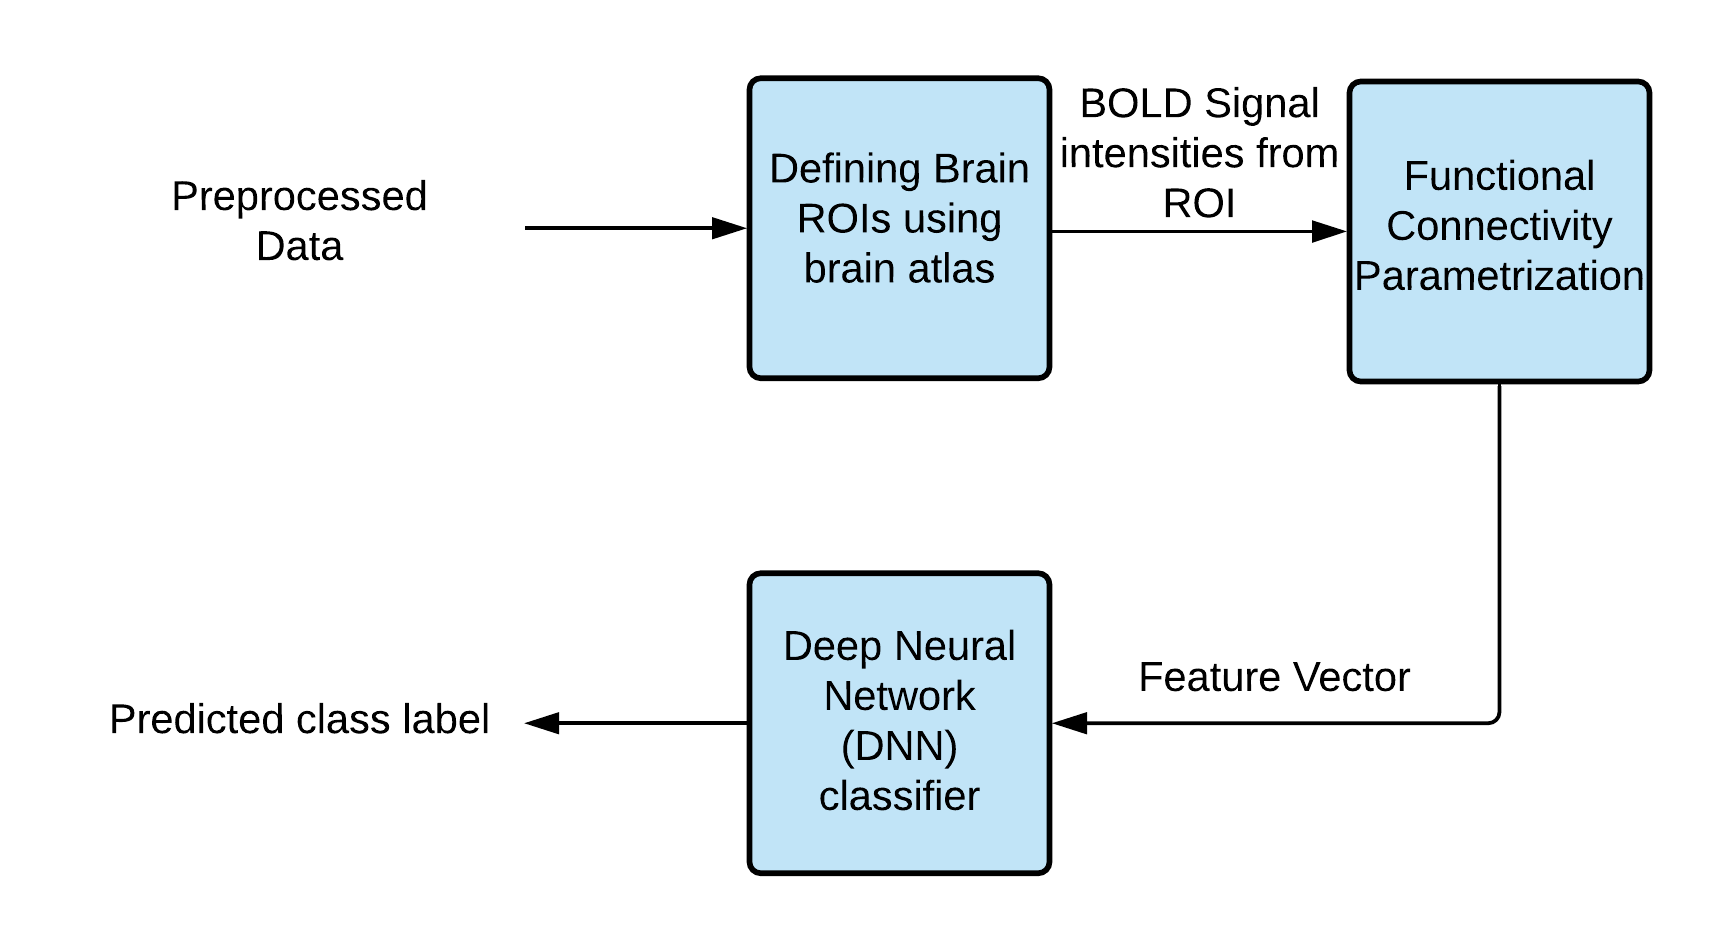
\includegraphics[width=\textwidth]{figures/figure1.1.png}
\caption{Block diagram of the ASD detection framework.}
\label{fig: 1.1}
\end{figure}

Our functional connectivity feature or functional connectome based ASD prediction framework comprises the following main
steps:\\
\begin{enumerate}
\item \textbf{Preprocessed Data:} Preprocessed rs-fMRI dataset are directly obtained from the CPAC preprocessing pipeline. Preprocessing is required for
nuisance signal removal, slice time correction, motion correction, skull stripping, etc.
\item \textbf{Defining brain ROIs using brain atlas:} Specific brain regions of interest (ROIs) are identified using
pre-defined brain atlases. Time-series signals or BOLD signal intensities are extracted only
from those regions that are defined by the respective brain atlas.
\item \textbf{Functional Connectivity Parametrization:} Functional interactions from time-series signals are
obtained from these ROIs and quantified using tangent space connectivity measure to
obtain a functional connectome or functional connectivity matrix.
\item \textbf{Classification:} Functional connectomes are flattened to produce one-dimensional
feature vectors and provided as input to a deep neural network classifier which predicts the class label i.e. autism or control.
\end{enumerate}


\section{Difficulties}
In this study, we worked with more than 800 subjects’ data (including ASD and control),
collected from 17 different international brain imaging laboratories worldwide belonging to
an age range of 7-64 years. The heterogeneity and complexity of such a dataset pose various
difficulties. The major difficulties are enlisted below:\\

\begin{enumerate}
\item \textbf{Reduced accuracy with larger dataset:} Many potential sources of uncontrolled
variation exist across studies and sites due to MRI acquisition protocols (such as
scanner type, imaging sequence), participant instructions (such as eyes open vs
closed), recruitment strategies (such as age group, IQ range, level of impairment,
treatment history and acceptable comorbidities) in \cite{abraham2017deriving}. Such variation affects
computer-aided diagnosis and provides low accuracy.

\item \textbf{Poor generalization with smaller dataset:} An accuracy above 0.9 is obtained
considering only a dozen subjects in \cite{arbabshirani2017single} and accuracy deteriorates consequently when
a larger dataset is considered. Thus, high accuracy can be achieved very conveniently
when using data from a single site. In contrast, such a procedure would not generalize
the problem efficiently.
\end{enumerate}

Hence, obtaining a reliable and fair accuracy using a heterogeneous dataset comprising a large number of participants/subjects is quite a challenge. 

\section{Applications}
The entire procedure of autism detection prevailing at present comprises a wide spectrum of
developmental monitoring, screening, comprehensive developmental evaluation including
parents interview, questionnaire and so on. This is a very complicated and comprehensive
method. Again, the absence of an objective medical test like a blood test, PET scan, EEG, CT
scan, etc is also responsible for a delayed autism diagnosis. The successful implementation of
deep learning in detecting ASD from brain fMRI data may be used for a wide range of
application:\\

\begin{enumerate}
\item Assistive technology for neuroscientists enabling them to obtain valuable insights
regarding autism spectrum disorder.
\item Visual evaluation of the functional characteristics and properties of the autistic brain.
\item Identifying neural activation patterns responsible for autism and associating those
patterns with physiological and psychological features would result in a more reliable
diagnosis.
\item By examining the contrast of rs-fMRI data of autistic and control brain the underlying
neural or biological basis of autism disorder can be unveiled and established.
\end{enumerate}

\section{Motivation}
To compete with the advancement of technologies in the neuroimaging field, there exists a
scope for improving the existing methods related to diagnosing neuropsychiatric disorders
utilizing functional MRI to produce results with more accuracy. The primary motivation
working behind this thesis can be listed as below:\\

\begin{enumerate}
    \item \textbf{To overcome existing limitations:} Most studies suffered from low accuracy and
huge training time problems using more than 800 subjects \cite{heinsfeld2018identification}. Our goal is to
achieve superior accuracy reducing the amount of training time thus alleviating
the limitations of previous work.
    \item \textbf{To introduce automated ASD diagnosis:} The traditional procedure for ASD diagnosis,
comprising an extensive battery of behavioural tests is less available than desired.
Many clinics may not have such facilities and experts capable of conducting such
assessments. Automated MRI based diagnosis can serve as a fruitful solution in
this case.
    \item \textbf{To reduce subjectivity in the field of diagnosis:} Automated computer-aided
diagnosis can be provided instead of a purely subjective and interview-based
diagnosis. It can also act as a supplement to the current diagnostic system.
    \item \textbf{Early detection of autism:} Early autism diagnosis is indispensable to prevent the
condition from intensifying further. This can be provided by MRI-based
diagnosis. It is a pain-free, non-invasive (requiring no medication, injection or
anaesthesia) diagnostic tool without side effects suitable for any age allowing
early diagnosis.
\end{enumerate}


\section{Contribution of the thesis}
Thesis or research works are conducted to fulfill a particular array of goals either by defining a new
methodology or by alleviating the limitations of the existing ones. In this thesis, the prime
objective is to focus on improving the accuracy of ASD detection using only rs-MRI data
while reducing training time. The primary contributions of this thesis are as follow:\\

\begin{enumerate}
\item Achieved a maximum accuracy of 88\% using only resting-state functional MRI (rs-fMRI) time-series data by the proposed scratch deep neural network model.
\item Reached the conclusion that the rarely used Bootstrap Analysis of Stable Clusters (\gls{BASC}) atlas using 122 ROIs yield a higher predictive power than other predefined atlases from comparative analysis.
\end{enumerate}

\section{Thesis Organization}
The remaining chapters are organized as follow:\\
\begin{itemize}
\item Chapter 2 gives a summary of previous research works, their contributions and
limitations in ASD detection using MRI data.
\item Chapter 3 describes the proposed methodology to detect ASD in detail with visual
representations wherever possible. In the proposed architecture, four different brain
atlases were used one at a time to perform the prediction task. The classifier used is
a deep neural network or \Gls{DNN}.
\item Chapter 4 describes the working dataset and the performance analysis for the
proposed method.
\item Chapter 5 contains the overall summary of this thesis, its limitations and future
recommendations as well.
\end{itemize}

\section{Conclusion}
In this chapter, a brief overview of our research work has been discussed. A summary of the
proposed framework, as well as the motivation behind this thesis and its applications, have
been represented. The research contributions along with the challenges faced are also
stated. In the next chapter, background, literature reviews and the current state of the problem
shall be provided.